% !TEX encoding = UTF-8 Unicode
\section{Systementwurf}
\subsection{Grundstruktur}
\begin{figure}[htbp]
\begin{center}
	\includegraphics[scale=0.3]{../graphics/DomainModel}
\caption{Die Grundstruktur von VSTForx}
\label{mainpat}
\end{center}
\end{figure}
Da es sich bei VSTForx um eine typische GUI-Anwendung handelt, wurde sich für das MVC-Architektur Pattern entschieden (siehe Abbildung \ref{mainpat}). 
\\\\
Lediglich einige Namen wurden angepasst:
\begin{itemize}
	\item Modell -> Processing
	\item View -> GUI\footnote{Anm.: da der ursprüngliche Arbeitstitel des Programmes ''PPI'' war, findet sich im Quelltext häufig die Bezeichnung ppiGui}
\end{itemize}
%%%%%%%%%%%%%%%%%%%%%%%%%%%%%%%%%%%%%%%%%%%%%%%%%%%%%%%%%%%%%%%
\subsection{Die Processing-Ebene}
\begin{figure}[htbp]
\begin{center}
	\includegraphics[scale=0.37]{../graphics/graph_overview}
\caption{Übersicht der Processing-Klassen und dessen Beziehungen zueinander}
\label{graphoverview}
\end{center}
\end{figure}
\paragraph{Die Graph-Klasse} Das Hauptelement in der Processing-Ebene ist der Graph. Mit ''Graph'' ist in diesem Fall nicht die Mathematische Struktur gemeint, sondern vielmehr die Repräsentation der ''Bühne'' (dessen Inhalte im Prinzip einen großen Graph darstellen). Er besteht aus allen Processing-Objekte die von der ''Bühne'' aus erzeugt werden. Die Elternklasse dieser Objektklassen ist, die PObject-Klase\footnote{PObject = Processing Object}(siehe Abbildung \ref{graphoverview}).  

\paragraph{Die G-Klasse}
Die G-Klasse repräsentiert das Mathematische Modell des (Prozess-)Graphen. Aus ihm wird, die in Abschnitt \ref{process} beschriebene Prozess-Liste erstellt. Ursprünglich war es geplant, das Graph-Modell mittels Kompositum-Muster zu implementieren. Da Knoten auf ihre Eltern-Knoten zugriff haben müssen (siehe Abschnitt Optimierung). Jeder Knoten verweist demnach auf seine Eltern- bzw. Kindknoten. Dies erwies sich in der Realisierung jedoch als sehr umständlich. Soll zum Beispiel ermittelt werden, welche Knoten nicht in die Prozesskette eingebunden sind, muss aufwändig durch die Knoten-Struktur traversiert werden, um jene Knoten auszuschließen. 
\\
Umgesetzt wurde schließlich die für Graphstrukturen übliche extrinistische Variante: die Knoten bzw. Kanten werden in einer Adjazent-Datenstruktur aufgenommen. Die Knoten selbst haben nur noch Zugriff, zu den (für den Ablauf benötigten) Eltern-Knoten. 
\\\\
Eine sehr gute Graph Implementation bietet die Boost Graph Library.
Sie bietet mehrere Vorteile: 
\begin{itemize}
	\item generische Implementierung (es kann durch Template-Parameter entschieden werden welche Datenstrukturen zur Speicherung der Knoten und Kanten verwendet werden soll)
	\item performant erweiterbar durch Template-Meta Programmiertechniken 
	\item große Anzahl an bereits Implementierten Algorithmen 
\end{itemize}
Ein Nachteil ist allerdings, da die Boost Library häufig Template-Meta Programmiertechniken verwendet, die lange Kompilationsdauer des Programmes.

\paragraph{Die Frames-Klasse}
Die Frames-Klasse ist ein (Mehrkanal)-Container für Sampleblöcke (siehe Abschnitt \ref{sampleblock}). Sie bietet außerdem Hilfsfunktionen wie: das Mischen mehrerer Kanäle zu Mono, Addition mehrerer Frames oder die Multiplikation um einen Faktor.

\paragraph{Die DCStream-Klasse}
Die DCStream-Klasse (DC=Delay Compensation) implementiert, die in Abschnitt \ref{Latenzproblem} beschriebene Lösung zum Latenzproblem. Eine Methode addFrames( Frames *frames, int numSamples, int delay ) bietet die Möglichkeit, Sampledaten eines Frames-Objektes, mit unterschiedlichen Versatzwerten in das DCStream-Objekt einzufügen. Über die Methode flush(int numSamples, Frames *target), wird der Sampledaten-Inhalt wieder in ein Frames-Objekt zurückgeschrieben. 

\paragraph{Die ProcessorNode-Klasse}
Die ProcessorNode-Klasse ist die Oberklasse aller Knoten, die vom Prozessgraphen (G) aufgenommen werden können. Die ProcessorNode-Klasse enthält die virtuellen Methoden: \emph{processNode()} und \emph{processFrames(Frames *fr)}.\\ 
Die Methode mixInputsToFrame() mischt alle Eingangs-Sampleblöcke, unter Verwendung der DCStream Klasse, in ein einzelnes Frames-Objekt. Die Methode processFrames() bearbeitet es (siehe Abbildung \ref{graphcomp}).
Die Methode popFrames() liefert schlußendlich die Ausgangs-Samplemenge. 
\\\\

\paragraph{Die ProcessAdapter-Klasse}
Würden alle gewünschten Module nur aus einem Eingang und einem Ausgang bestehen, wäre es völlig ausreichend, die Modulfunktionen in einem Knoten zu implementieren. Da jedoch Module implementiert werden müssen die mehrere Ein-/Ausgänge verwenden, ist die Umsetzung etwas aufwändiger. Um zum Beispiel mehreren Ausgängen, (=mehrere Kindknoten) unterschiedliche Frames zu liefern zu können, bräuchte ein Knoten die Information, von welchem Kinds-Knoten aus die popFrames() Methode aufgerufen wurde. Eine solche Implementierung wäre sehr fehleranfällig und schwer zu nachzuvollziehen. 
\\\\
Eine bessere Lösung ist, dass Knoten selbst die Ein- und Ausgänge darstellen (siehe Abbildung \ref{graphcomp}). Erzeugt und verwaltet werden diese vom Modul, der ProcessAdapter-Klasse. Ein zusätzlicher Knoten-Typ, der ProcessAdapterNode, sorgt dafür das der Aufruf processNode(), an das jeweilige Eltern-Modul verwiesen wird (siehe Abbildung \ref{lanes}).

\paragraph{Optimierung} 
Effizient wäre es, nach jeder Knoten-bearbeitung den Zeiger des Frames-Objekt weiterzureichen. Dies funktioniert allerdings nur  solange, wie Knoten in Serie verkettet sind. Bei einer Parallel-Verkettung ist es notwendig das Frames-Objekt, einmal für jede Abzweigung zu kopieren. Ziel ist es, so viele Kopiervorgänge wie möglich zu sparen. Dies wird erreicht, indem nur dann kopiert wird wenn es wirklich notwendig ist: wenn ein Knoten mehr als ein Kindknoten hat. \\\\
Zur Umsetzung wurde ein Stack-Mechanismus verwendet. Die Ausgabeframes eines Knotens, gelangen über die Methode pushAndCopy(Frames*) in den Stack. Sollte eine Knoten nur ein Kindknoten haben, wird der übergebene Frames-Zeiger der pushAndCopy() Methode, im Stack aufgenommen. Bei mehr als einem Kindknoten, wird zusätzlich Anzahl(Kindknoten) - 1 mal das Frames Objekt kopiert und im Stack aufgenommen. 
\\\\
Die Kindknoten können nun über die Methode popFrames(), ein Frames Objekt als Eingabe-Sampleblockmenge abholen.

\begin{figure}[htbp]
\begin{center}
	\includegraphics[scale=0.35]{../graphics/processingSeq}
\caption{Beispiel-durchlauf eines Prozessaufrufes von VSTForx}
\label{lanes}
\end{center}
\end{figure}

\begin{figure}[htbp]
\begin{center}
	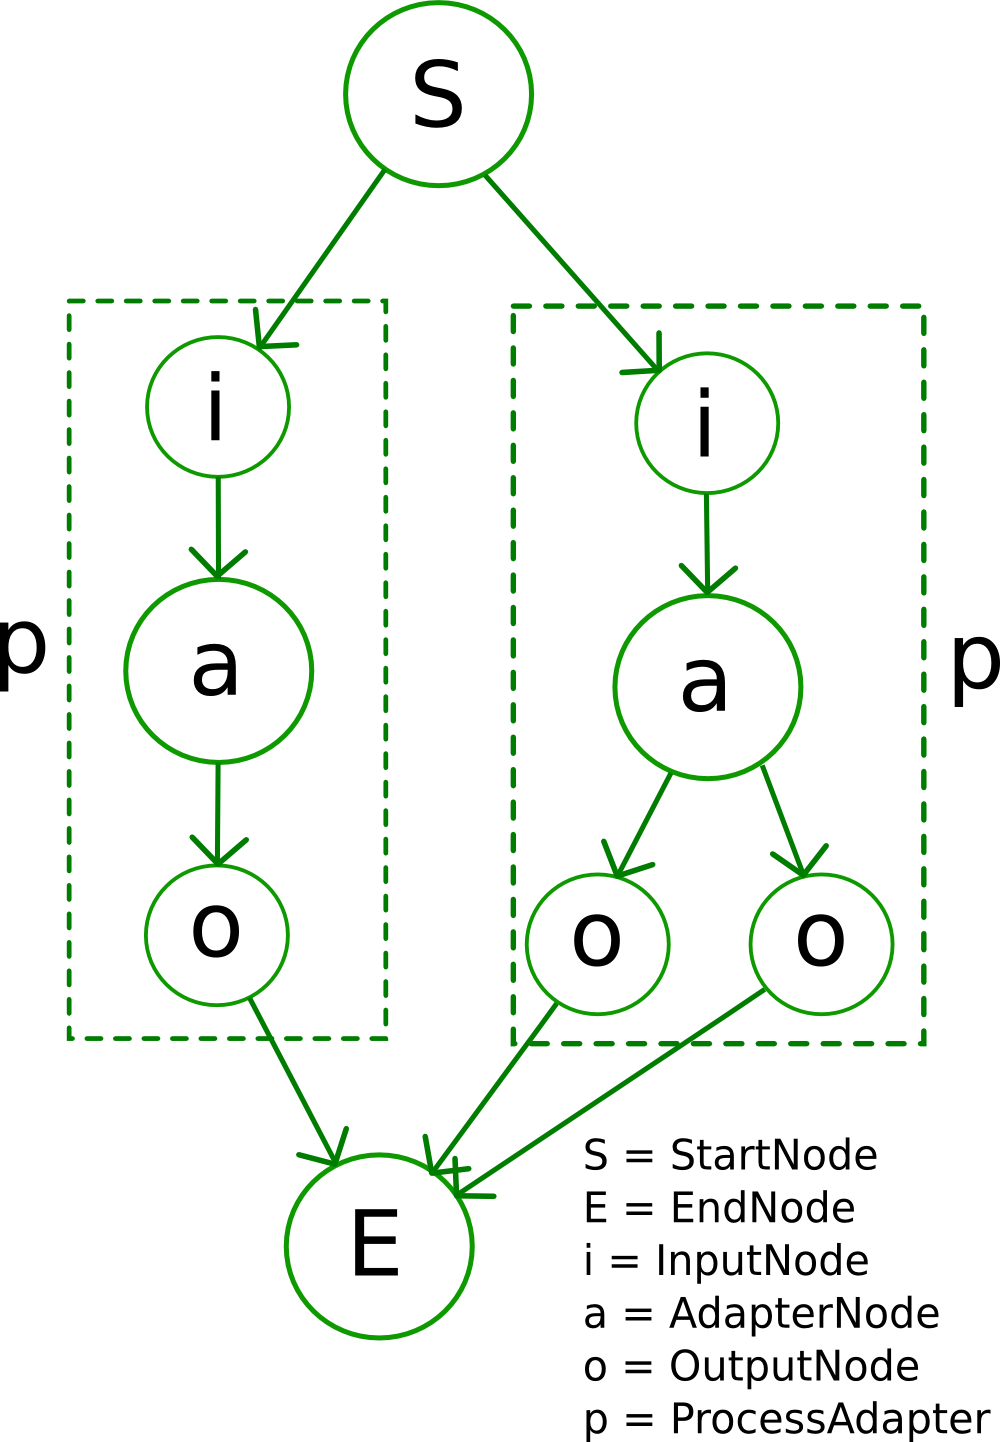
\includegraphics[scale=0.12]{../graphics/graphcomp}
\caption{Beispiel Graph bestehend aus Processing-Klassenobjekten}
\label{graphcomp}
\end{center}
\end{figure}

\subsubsection{Parameter}
Es wäre naheliegend, die Implementation der Parameter und dessen Verbindungsmöglichkeiten, ebenfalls mittels eines Graph-Modells umzusetzen. Es gibt aber, im Gegensatz zum Prozess-Graph, eine entscheidende Vereinfachung: es bestehen keine Abhängigkeiten. Wird ein Parameter verändert, ist es egal in welcher Reihenfolge die verbundenen Nachbarparameter, über die Änderung informiert werden.
So wurde sich für ein einfachen Observer-Entwurf\footnote{im Unterschied zum GoF-Observer, existiert hier jedoch keine Observer Schnittstelle} entschieden (siehe Abbildung \ref{parameterModel}).
\paragraph{ParameterConnection}
Die ParameterConnection-Klasse entspricht dem Observer-Objekt. Jedes Parameter-Objekt enthält eine unbestimmte Menge an ParameterConnection-Objekten. Wird ein Parameterwert verändert, werden diese Objekte benachrichtigt. Zu beachten ist, dass Parameterverbindungen Bidirektional sind. So muss für eine Parameter-Verbindung (A<->B), A sowie B ein ParameterConnection-Objekt (A->B, B->A) enthalten. 

\paragraph{ConnectionOperator}
Neben dem Nachbarparameter enthält ein ParameterConnection-Objekt eine unbestimmte Menge an ConnectionOperatoren. Diese bearbeiten den zu übermittelnden Parameterwert. Auch hier ist die Bidiretionalität zu beachten. Für eine Parameter-Verbindung (A<->B), muss die Verbindung(B->A) die Inverse-Operation zur Verbindung (A->B) enthalten. Den Inverse-ConnectionOperator liefert die Methode: getInverseOperator().
\paragraph{HasParameter}
Die Schnittstelle HasParameter, ermöglicht den zugriff auf eine unbestimmte Menge an Parameterobjekten. So wird diese Schnittstelle, unter anderem, von allen Modulen und den Plugins implementiert. 
\begin{figure}[htbp]
\begin{center}
	\includegraphics[scale=0.45]{../graphics/ParameterOverview}
\caption{Parameter-Klassen Modell}
\label{parameterModel}
\end{center}
\end{figure}
%%%%%%%%%%%%%%%%%%%%%%%%%%%%%%%%%%%%%%%%%%%%%%%%%%%%%%%%%%%%%%%
\subsection{Die GUI Ebene}
\paragraph{PpiEditor}
Die PpiEditor-Klasse implementiert, die von dem Vst-Gui SDK vorgegebene AEffGUIEditor-Klasse. Sie dient der Kommunikation zwischen Hostanwendung und Plugin-Editor.
\paragraph{CView}
Die CView-Klasse ist die Oberklasse aller graphischen Elemente im Vst-Gui SDK. Sie besteht aus einem Rechteckigen Bereich und enthält die Methode draw(CDrawContext *cn). Über diese können mittels übergebenen DrawContext, im sichtbaren Bereich Zeichenoperationen ausgeführt werden.
\paragraph{CircuidView}
Die CircuidView-Klasse repräsentiert die ''Bühne'' der GUI.
Zu beginn der Entwicklung stand der Autor vor der Entscheidung, die Bühnedarstellung nach Vst-Gui SDK Methodik zu gestalten oder eine eigene Implementierung zu verwenden. So könnte jedes Bühnenobjekt einen eigenen CView-Bereich darstellen. Was aus Sicht des Vst-Gui SDKs durchaus logisch wäre, da dort alle graphischen Elemente, wie Regler und Knöpfe, als CView-Klasse implementiert sind. 
\\\\
Es wurde sich allerdings dagegen entschieden. So ist einzig die CircuidView-Klasse eine CView-Klasse. Sie ist für das Zeichnen der Bühne und allen enthaltenen Objekten verantwortlich. Die Gründe für diese Entscheidung waren:
\begin{itemize}
	\item das Vst-Gui SDK wurde nicht für dynamische Oberflächen mit frei beweglichen Objekten entworfen (dargestellt werden üblicherweise Konsolen mit fest positionierten Bedienelementen)
	\item die schlechte Dokumentation des Vst-Gui SDKs (Erschließung hauptsächlich nach ''trial and error'' Prinzip)
	\item weniger direkte Abhängikeiten zum Vst-Gui SDKs (was eine eventuelle Immigration zu einem anderen/besseren Framework erleichtern würde)
\end{itemize}
\paragraph{GObject}
Die GObject-Klasse ist die Oberklasse, aller Objekte die von der CircuidView aufgenommen werden können. Sie bildet das Gegenstück zur PObject Klasse.
\paragraph{GProcessModule}
Die GProcessModule-Klasse ist die graphische Repräsentation der ProcessAdaptor-Objekte.
\paragraph{GIONode}
Die GIONode-Klassen repräsentieren die Input-/OutputNode Objekte.
\paragraph{GConnection}
Die GConnection-Klassen repräsentieren die Verbindungen zwischen den GObjecten.
\paragraph{CViewWrapper}
Wie bereits beschrieben, implementiert die CircuidView-Klasse die Bühnedarstellung, unabhängig von den CView-Klassen. Die CircuidView nimmt ausschließlich GObject-Objekte auf. Dies bedeutet jedoch, dass Vst-Gui SDK Steuerungs-Elemente, nicht mit der CircuidView verwendet werden können. Diesen Nachteil behebt die CViewWrapper-Klasse. Sie hüllt ein CView-Objekt in ein GObject-Objekt. Über ein Template-Parameter wird festgelegt, welche GObject-Klasse Oberklasse ist. Somit ist es möglich, Eine CView-Klasse mit den Eigenschaften von GCircle zu umhüllen.
\begin{figure}[htbp]
\begin{center}
	\includegraphics[scale=0.45]{../graphics/gui_overview}
\caption{Parameter-Klassen Modell}
\label{parameterModel}
\end{center}
\end{figure}
%%%%%%%%%%%%%%%%%%%%%%%%%%%%%%%%%%%%%%%%%%%%%%%%%%%%%%%%%%%%%%%
\subsection{Die Control Ebene}
\paragraph{CircuidControl}
\paragraph{FrontController}
%gründe für mvc